\documentclass[tikz,border=5mm]{standalone}

\begin{document}    
    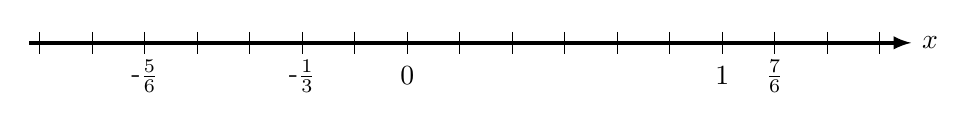
\begin{tikzpicture}[line join=round,scale=4]
        \newcommand*{\ar}{1/6}
        \draw[very thick,black,-latex]   (-1.2,0) -- (1.6,0) node[right] {$x$};     
        \foreach \x in {-7,-6,...,9}
        \draw (\ar*\x,1pt) -- (\ar*\x,-1pt);
        \foreach \x/\y in {-5*\ar/{-$\frac56$},-2*\ar/{-$\frac13$},0/{0},1/{1},7*\ar/{$\frac76$}}
        \node at (\x,-3pt) () {\y}; 
    \end{tikzpicture}
\end{document}